% ===== 原文 pp.34--38 =====

% [原文 p.34]
\para{BPS 谱。} $\lambda$ 的围道积分给出 $\lambda=x\,\dd z=\pm\sqrt{u_2}\,\dd z$ 在极点 $z=0,1,\infty$ 处留数的整数\footnote{我们忽略留数定理中的因子 $2\pi\ii$。}线性组合。由构造，这些留数是 $\pm m_1,\pm m_2,\pm m_3$，故我们发现 BPS 态的质量（更确切地说，中心荷）取 $Z=f_1m_1+f_2m_2+f_3m_3$ 的形式，其中 $f_1,f_2,f_3\in\Z$。另一方面，三基本表示半超多重态只有 $\pm m_1\pm m_2\pm m_3$ 的整数线性组合这样的 BPS 态：这施加了进一步限制 $f_1=f_2=f_3\bmod 2$。tinkertoy $T_2$ 是否也有这个限制？

在 3.3 小节我们学到，M 理论指导我们只把 $\lambda$ 沿 $\Sigma\subset T^*C$ 中那些可以写成某个二维曲面 $D\subset T^*C$ 的边界 $\gamma=\partial D$ 的围道积分。

\begin{exercise}{4.4}
1. 先取 $D$ 为绕某个穿刺点的小圆乘以连接 $\Sigma$ 两片的区间。它的边界是一对圆，拾取两次相同的留数 $m_i$（来自不同的片）。由此推出 $2m_1,2m_2,2m_3$ 以及它们的一切整数线性组合都在谱中。

2. 接着取 $D$ 使得 $\partial D$ 是一条从一个分支点到另一个分支点（在一片上前进）再经另一片返回的围道。注意 $\partial D$ 可以形变为停留在同一片上并绕住割线的围道。由此推出 $\lambda$ 的积分是组合 $\pm m_1\pm m_2\pm m_3$ 之一（围道每侧有三个极点），并断定 $T_2$ 的 BPS 谱包含一切 $Z=f_1m_1+f_2m_2+f_3m_3$（$f_1=f_2=f_3\bmod 2$）。

3. （数学。）对任何边界满足 $\partial D\subset\Sigma$ 的 $D\subset T^*C$，考虑投影 $\pi: T^*C\to C$，并推断 $\pi(\partial D)=\partial(\pi(D))$ 不能包围一个极点。由此断定 $T_2$ 的 BPS 谱恰好就是三基本表示半超多重态的谱。
\end{exercise}

一般地，所有这些 BPS 粒子都是有质量的，因此低能理论是空的。一个有意思的情形是极限 $m_2\to\pm(m_1\pm m_3)$，此时三基本表示半超多重态中的四个超多重态之一变成无质量的。于是 SW 曲线退化，因为两个分支点相撞：确实，$u_2$ 有（(4.8) 中的）二重根
\begin{equation}
  z^2(z-1)^2u_2(z)=(m_1\pm z\,m_3)^2.
  \tag{4.10}
\end{equation}
我们在上面习题第 2 点考虑过的围道缩为零尺寸，而 $\lambda$ 本身保持有限，故积分确实为零，与质量消失相容。我们将对更复杂的理论跑这类容易的自洽性检验。

% [Tutor Note: p.34 式 (4.10) 的验算：把 $m_2^2=(m_1+m_3)^2$ 代入 (4.8) 右端，得 $-(z-1)m_1^2+z(m_1+m_3)^2+z(z-1)m_3^2=-zm_1^2+m_1^2+zm_1^2+2zm_1m_3+zm_3^2+z^2m_3^2-zm_3^2=m_1^2+2zm_1m_3+z^2m_3^2=(m_1+zm_3)^2$ ✓（取另一符号得 $(m_1-zm_3)^2$）。这正是“$P(z)$ 有二重根 ⇔ 两分支点相撞 ⇔ 某个超多重态变无质量”的代数体现。]

\subsection{4d $\cN=2$ $\mathrm{SU}(2)$ $N_f=4$ SQCD}

讲了这么多一般性之后，让我们来研究第一个有意思的具体理论：球面上带四个驯服穿刺点的 $\cX(\fsu(2))$ 的 Coulomb 分支、SW 曲线与 S 对偶性。

\para{识别 4d 理论（标题里已有剧透）。} 我们把四个穿刺点放在二维球面 $\C P^1$ 上的 $z_1=0$、$z_2=q$、$z_3=1$、$z_4=\infty$。四孔球面的三个退化极限 $q\to0,1,\infty$ 对应于把穿刺点两两聚拢的一切方式。

% [原文 p.35]
由于这三个极限只差穿刺点的置换，我们集中看 $q\to0$。在这个极限下，我们按一般理由预期该 4d 理论由两个 tinkertoy $T_{\fsu(2)}$ 和一个 $\mathrm{SU}(2)$ 矢量多重态组成，后者把每个 tinkertoy 的一个 $\mathrm{SU}(2)$ 味对称性规范化。规范化之后，每个 tinkertoy 仍应至少带有与其剩余两个穿刺点相关联的 $\fsu(2)\times\fsu(2)$ 味对称性。我们可以把这画成一个（广义的）箭图（generalized quiver），使所有对称性都显式：
\begin{equation}
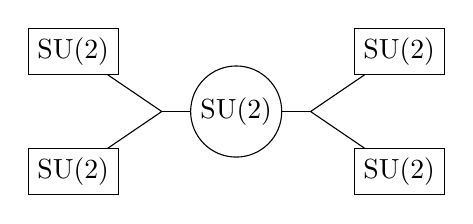
\begin{tikzpicture}[scale=0.9,baseline=(current bounding box.center)]
  \node[draw,rectangle] (l1) at (-2.3,0.85) {$\mathrm{SU}(2)$};
  \node[draw,rectangle] (l2) at (-2.3,-0.85) {$\mathrm{SU}(2)$};
  \node[draw,circle,inner sep=2pt] (g) at (0,0) {$\mathrm{SU}(2)$};
  \node[draw,rectangle] (r1) at (2.3,0.85) {$\mathrm{SU}(2)$};
  \node[draw,rectangle] (r2) at (2.3,-0.85) {$\mathrm{SU}(2)$};
  \draw (l1) -- (-1.05,0) -- (l2);
  \draw (-1.05,0) -- (g);
  \draw (r1) -- (1.05,0) -- (r2);
  \draw (1.05,0) -- (g);
\end{tikzpicture}
\tag{4.11}
\end{equation}
这里圆节点表示规范群，方块节点表示味对称性。每个“岔口”（图中画成 $>$ 形的接点）代表我们钟爱的 tinkertoy $T_2$，即三基本表示半超多重态，也就是四个超多重态按 $\mathrm{SU}(2)$ 规范群的两个双重表示来变换。

于是我们从左侧岔口得到两个味、从右侧岔口得到两个味，故该理论是 $N_f=4$ 的 $\mathrm{SU}(2)$ SQCD。虽然 (4.11) 中每个 tinkertoy 在规范化 $\mathrm{SU}(2)$ 之后有 $\mathrm{Spin}(4)$ 味对称性，但整个理论有 $N_f=4$ 个处于同等地位的 $\mathrm{SU}(2)$ 双重态，因而有比 $\mathrm{Spin}(4)^2$ 更大的 $\mathrm{Spin}(8)$ 味对称性。这个 4d 理论的对称性只在 $C$ 收缩为一点的极限下才涌现。

% [Tutor Note: p.35 式 (4.11) 的箭图按 STYLE_GUIDE 6bis 用 TikZ 重画（原文：中央椭圆节点 $\mathrm{SU}(2)$ 接左右两个“$>$”形岔口，每个岔口连两个方框 $\mathrm{SU}(2)$）。核对味计数：每个 $T_2$ 贡献 $\mathrm{SU}(2)^3$，其中一个被规范（圆节点），剩下两个方框；左右各一，故 $N_f=2+2=4$。核对 $\mathrm{Spin}(8)$：4 个 $\mathrm{SU}(2)$ 双重态 = 8 个 Weyl 费米子 ⇒ 味群 $\mathrm{SO}(8)$（旋量为 $\mathrm{Spin}(8)$），而每个 tinkertoy 单独只剩 $\mathrm{Spin}(4)=\mathrm{SU}(2)^2$，故 $\mathrm{Spin}(8)\supset\mathrm{Spin}(4)^2$ 是更大的对称性。]

\para{Coulomb 分支。} 我们把 $m_1,m_2,m_3,m_4$ 记为这些穿刺点各自的质量参数（在 (4.2) 或 (4.4) 的意义下）。该 4d 理论的 Coulomb 分支真空由全纯二次微分 $\phi_2(z)$ 参数化：这些微分在每个穿刺点处有二阶极点 (4.2)（无质量情形下为一阶 (4.4)），且没有其他极点。无穷远处的穿刺点翻译为 $z\to\infty$ 时的条件：
\begin{equation}
  \phi_2(z)=\left(\frac{m_4^2}{z^2}+O\!\left(\frac{1}{z^3}\right)\right)\dd z^2.
  \tag{4.12}
\end{equation}
我们在下一个习题中参数化可能的 $\phi_2(z)$，先从无质量情形 $m_1=m_2=m_3=m_4=0$ 开始，此时 $\phi_2$ 只有一阶极点。

\begin{exercise}{4.5}
1. 找出在 $0,q,1,\infty$ 处有一阶极点且没有其他极点的所有二次微分 $\phi_2(z)=u_2(z)\dd z^2$。（提示：把它写成 $u_2(z)=f(z)/(z(z-q)(z-1))$ 后，换到 $w=1/z$ 变量以得到对 $f(z)$ 的多项式界，然后使用前面提到的 Liouville 定理。）

2. 找出一个二次微分 $\phi_2$，使其在 $i=1,2,3$ 处具有首项行为 $m_i^2/(z-z_i)^2$、在无穷远处具有 $m_4^2/z^2$（按 (4.12)）。与无质量情形合并，推出所有这样的二次微分。
\end{exercise}

我们得到一维 Coulomb 分支 $\cB=\C$，其真空为\footnote{参数化 Coulomb 分支的变量 $u$ 可以自由重定义，所以你在习题 4.5 中得到的表达式可能略有不同。}
\begin{equation}
  \phi_2=u_2\dd z^2,
  \qquad
  u_2(z)=\frac{\frac{q}{z}m_1^2+\frac{q(q-1)}{z-q}m_2^2+\frac{z-q}{z-1}m_3^2+zm_4^2-u}{z(z-q)(z-1)}
  \tag{4.13}
\end{equation}

% [Tutor Note: p.35 式 (4.13) 的极点核对（逐点代入即可）：$z\to0$ 时分子首项 $(q/z)m_1^2$、分母 $\sim zq(-1)$，故 $u_2\sim m_1^2/z^2$ ✓；$z\to q$ 时分子 $\sim\frac{q(q-1)}{z-q}m_2^2$、分母 $\sim q(z-q)(q-1)$，故 $\sim m_2^2/(z-q)^2$ ✓；$z\to1$ 时分子 $\sim\frac{1-q}{z-1}m_3^2$、分母 $\sim(1-q)(z-1)$，故 $\sim m_3^2/(z-1)^2$ ✓；$z\to\infty$ 时分子 $\sim zm_4^2$、分母 $\sim z^3$，故 $\sim m_4^2/z^2$ ✓，与 (4.12) 一致。]

% [原文 p.36]
这些真空由 $u\in\cB=\C$ 标记。一项零阶检验（用来确认我们没有走偏）是：我们得到了 $\mathrm{SU}(2)$ SQCD（$N_f=4$ 味）Coulomb 分支的正确维数（即 1）。

\para{退化极限。} 当 $q\to0$ 时曲面退化，我们应当在某种适当的意义下得到两个断开的三孔球面。对 $|q|,|z|\ll1$ 且质量固定时，(4.13) 的行为是
\begin{equation}
  \phi_2(z)\simeq
  \frac{-\frac{q}{z}m_1^2+\frac{q}{z-q}m_2^2+u}{z(z-q)}\dd z^2,
  \tag{4.14}
\end{equation}
这恰好是带三个驯服穿刺点（质量平方为 $m_1^2$、$m_2^2$ 与 $u$）的球面上的二次微分。同样，对 $|q|\ll|z|,1$，(4.13) 的行为是带三个穿刺点（质量平方为 $u$、$m_3^2$ 与 $m_4^2$）的三孔球面上的二次微分。这与我们在 4.1 小节引入驯服穿刺点的方式一致。

% [Tutor Note: p.36 式 (4.14) 的来历：在 $|q|,|z|\ll1$（$z/q$ 固定）的区域，$z-1\simeq-1$、$q(q-1)\simeq-q$，故 (4.13) 的分母 $z(z-q)(z-1)\simeq-z(z-q)$；分子中 $\frac{z-q}{z-1}m_3^2\simeq-(z-q)m_3^2$ 与 $zm_4^2$ 分别是 $O(\max(|z|,|q|))$、$O(|z|)$，比主导项（$m_1^2,m_2^2$ 的 $O(1/|q|)$ 与 $u$ 的 $O(1)$）小，可略去，整理即得 (4.14)。几何上：四孔球面退化时，$z=0$（质量 $m_1^2$）与 $z=q$（$m_2^2$）连同管子（质量平方 $u$）构成一个三孔球面，$z=1$（$m_3^2$）与 $z=\infty$（$m_4^2$）连同同一根管子构成另一个三孔球面；这与原文接下来“$|q|\ll|z|,1$ 时质量平方为 $u,m_3^2,m_4^2$”的说法一致。]

由于质量是矢量多重态标量的背景值，我们从 (4.14) 学到识别
\begin{equation}
  u=\frac12\left\langle\Tr\phi^2\right\rangle
  \tag{4.15}
\end{equation}
在弱耦合极限 $|q|\ll1$ 下，其中 $\phi$ 是对应 $\mathrm{SU}(2)$ 规范群的（动力学）矢量多重态标量。换言之，$u$ 就是 SQCD 的 Coulomb 分支通常所用的参数化。

\para{Seiberg--Witten 曲线。} 现在回到一般的 $q$。SW 曲线与微分由 $\Sigma=\{(x,z)\in T^*\C P^1\mid x^2=u_2(z)\}$ 与 $\lambda=x\,\dd z$ 定义。

曲线 $\Sigma$ 是 $\C P^1$ 的分歧二重覆盖。它有多少个分支点？分支点是两片 $x=\pm\sqrt{u_2}$ 重新接合的地方，即 $u_2=0$ 的地方。这发生在多项式 $z^2(z-q)^2(z-1)^2u_2(z)$ 的（一般地）四个根处，而它是四次多项式。总之，$\Sigma$ 绕球面两圈，有四个分支点，由两条分支割线相连。因此它在拓扑上是一个环面。除了这些分支割线之外，我们还在 $0,q,1,\infty\in\C P^1$ 处有四个穿刺点，于是在 $\Sigma$ 上有八个点使 SW 微分 $\lambda$ 发散：
\begin{equation}
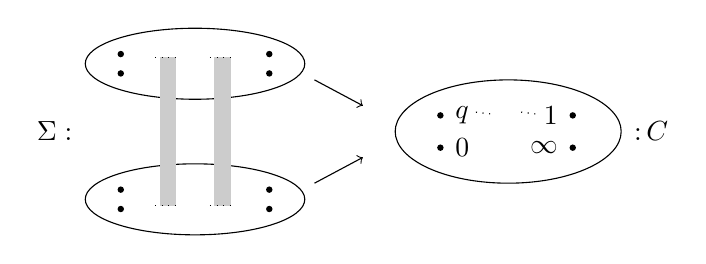
\begin{tikzpicture}[scale=0.82,baseline=(current bounding box.center)]
  \draw (1.9,1.05) ellipse (1.7 and 0.55);
  \fill (0.75,1.2) circle (0.05);
  \fill (0.75,0.9) circle (0.05);
  \fill (3.05,1.2) circle (0.05);
  \fill (3.05,0.9) circle (0.05);
  \draw (1.9,-1.05) ellipse (1.7 and 0.55);
  \fill (0.75,-0.9) circle (0.05);
  \fill (0.75,-1.2) circle (0.05);
  \fill (3.05,-0.9) circle (0.05);
  \fill (3.05,-1.2) circle (0.05);
  \draw[fill=gray!40,draw=none] (1.35,-1.15) rectangle (1.6,1.15);
  \draw[fill=gray!40,draw=none] (2.2,-1.15) rectangle (2.45,1.15);
  \draw[dotted] (1.28,1.15)--(1.67,1.15);
  \draw[dotted] (1.28,-1.15)--(1.67,-1.15);
  \draw[dotted] (2.13,1.15)--(2.52,1.15);
  \draw[dotted] (2.13,-1.15)--(2.52,-1.15);
  \node[left] at (0.15,0) {$\Sigma:$};
  \draw[->] (3.75,0.8)--(4.5,0.4);
  \draw[->] (3.75,-0.8)--(4.5,-0.4);
  \draw (6.75,0) ellipse (1.75 and 0.8);
  \fill (5.7,0.25) circle (0.05);
  \node[right] at (5.78,0.25) {$q$};
  \fill (5.7,-0.25) circle (0.05);
  \node[right] at (5.78,-0.25) {$0$};
  \fill (7.75,0.25) circle (0.05);
  \node[left] at (7.67,0.25) {$1$};
  \fill (7.75,-0.25) circle (0.05);
  \node[left] at (7.67,-0.25) {$\infty$};
  \draw[dotted] (6.25,0.3)--(6.5,0.27);
  \draw[dotted] (6.95,0.3)--(7.2,0.27);
  \node[right] at (8.55,0) {$\colon C$};
\end{tikzpicture}
\tag{4.16}
\end{equation}

% [Tutor Note: p.36 式 (4.16) 的线描图（两个灰色带 = 两条分支割线，四个黑点 = 四个穿刺点）按 6bis 用 TikZ 重画。亏格核对（Riemann--Hurwitz）：$\Sigma$ 是 $\C P^1$ 的二重分歧覆盖、有 $R=4$ 个二阶分支点，故 $2g-2=2(2\cdot0-2)+4=0$，即 $g=1$，与正文“拓扑上是环面”一致；八个点 = 四个穿刺点 × 两片。]

\begin{exercise}{4.6}
1. 通过作坐标变换 $x=\tilde x/z+m_2/(z-q)+m_3/(z-1)$，把曲线 $x^2=u_2$ 重写成在 $z=0,q,1$ 处只有简单极点的形式。证明 $\tilde\lambda:=\tilde x\,\dd z/z$ 与 SW 微分 $\lambda=x\,\dd z$ 相差一个与 $u$ 无关的项，其围道积分（留数）是质量的线性组合。回忆 BPS 质量公式 $\oint\lambda=n\,a+m\,a_D+f_i m_i$，并检查把 $\lambda$ 换成 $\tilde\lambda$ 相当于对味荷作一个重定义。至多作一些简单的坐标变换，或许就能与
% [原文 p.37]
更常规的 $\mathrm{SU}(2)$ $N_f=4$ SQCD 的 SW 曲线与微分表达式 [123] 相符\footnote{我还没去核对 Martone 在他的讲义里用的是哪种形式。}。这一相符确认了我们正确识别了 tinkertoy $T_{\fsu(2)}$。
\end{exercise}

% [Tutor Note: p.37 上接 p.36 的习题 4.6（跨页句由本块写完）。此处的“相符”指的是把 $\tilde\lambda$ 与 [123] 中 $\mathrm{SU}(2)$ $N_f=4$ SQCD 的标准 SW 微分比较：坐标变换 $x=\tilde x/z+m_2/(z-q)+m_3/(z-1)$ 给出 $\tilde\lambda=\tilde x\,\dd z/z=\lambda-m_2\,\dd z/(z-q)-m_3\,\dd z/(z-1)=\lambda-\dd\big(m_2\log(z-q)+m_3\log(z-1)\big)$；后两项是全微分，沿闭圈的积分为 $2\pi\ii$ 乘质量的整数组合，故把 $\lambda$ 换成 $\tilde\lambda$ 只平移味荷 $f_i$ 而不改变 BPS 谱。这正是原文“与 $u$ 无关的项”“对味荷作重定义”的确切含义。]

\para{Coulomb 分支上的奇点。} 正如我们在第 24 页描述过的，低能理论一般是 4d $\cN=2$ 阿贝尔规范理论，其矢量多重态标量生活在 Coulomb 分支 $\cB$ 中。对 $u$ 与质量的一般取值，我们于是得到 $\mathrm{U}(1)$ 矢量多重态；但在参数的某些特殊取值处，一些分支点可能相撞，从而导致有意思的低能行为。我们在研究 tinkertoy 时已经在 (4.10) 附近看到过这一点：我们找到了质量的某些特殊取值，使 SW 曲线的一对分支点相撞。这一相撞使某条围道缩为零尺寸，从而产生一个无质量 BPS 粒子，它仍留在 IR 理论中。对 SQCD，这类分支点相撞会通过增加一个或多个在低能 $\mathrm{U}(1)$ 下带电的无质量超多重态，使 IR 理论变得更丰富。

\begin{exercise}{4.7（论判别式）}
次数为 $d$ 的多项式 $P(z)=p_d\prod_{a=1}^{d}(z-z_a)$ 的判别式是 $\Delta_P=p_d^{2d-2}\prod_{a<b}(z_a-z_b)^2$。按构造，它恰在 $P(z)$ 有二重根时为零。已知 $\Delta_P$ 可以写成 $P(z)=\sum_{j=0}^{d}p_jz^j$ 的系数的 $2d-2$ 次多项式。对二次多项式验证这一点。
\end{exercise}

我们的问题是：$P(z)=z^2(z-q)^2(z-1)^2u_2(z)$（即 (4.13) 中显式给出的四次多项式）何时有二重根（也就是两个分支点何时相撞）。此时判别式 $\Delta_P$ 是 $P$ 的系数的 6 次多项式。由于 $P$ 线性依赖于 $u$，我们发现 $\Delta_P$ 是 $u$ 的 6 次多项式（其首项系数经查非零）。因此我们应当预期 Coulomb 分支上有 6 个奇点。

% [Tutor Note: p.37 的计数核对：判别式关于系数的次数为 $2d-2$（$d=4$ 时即 6）；而 $P(z)=z^2(z-q)^2(z-1)^2u_2(z)$ 对 $u$ 是线性的（$u$ 只以 $-u$ 的形式出现在 $u_2$ 的分子里），故 $\Delta_P$ 是 $u$ 的 6 次多项式，一般有 6 个根，即 Coulomb 分支上 6 个奇点。$2d-2$ 的快速验算：对 $d=2$，$P=p_2(z-z_1)(z-z_2)$，$\Delta_P=p_2^{2}(z_1-z_2)^2=p_1^2-4p_0p_2$ 确实是系数的 2 次式 ✓。这与后文“弱耦合看到 4 个、剩下 2 个”（4+2=6）吻合。]

其中四个可以在弱耦合极限下（质量固定）具体看到。此时 $\phi_2$ 大致由每个裤子上各自的二次微分给出，而这些裤子由一段 $\phi_2$ 近似为常数的长管子连接，见 (4.14)。每个三孔球面有两个 $\phi_2$ 的零点，因而对应 SW 曲线的一条分支割线。为确定起见，考虑质量平方为 $m_1^2,m_2^2,u$ 的那个裤子。只要质量参数的任一组合 $\pm m_1\pm m_2\pm\sqrt{u}$ 为零，它的分支割线就缩为零尺寸。于是我们得到 Coulomb 分支六个奇异点中的四个：
\begin{equation}
  u=(m_1\pm m_2)^2+O(q)
  \qquad\text{与}\qquad
  u=(m_3\pm m_4)^2+O(q).
  \tag{4.17}
\end{equation}
剩下两个点不那么容易从 class S 理论的显式二次微分 (4.13) 定出来，部分原因是它们对应于落在上述分解中不同裤子里的分支点相撞。一项冗长的级数展开表明，在
\begin{equation}
  u=\pm2\left(q(m_2^2-m_1^2)(m_3^2-m_4^2)\right)^{1/2}+O(q)
  \tag{4.18}
\end{equation}
处，两个分支点在 $z=\mp2\left(q(m_2^2-m_1^2)/(m_3^2-m_4^2)\right)^{1/2}+O(q)$ 处相撞，符号与 $u$ 的符号相关联。\footnote{若能从我们的 6d 构造更好地理解这些公式，那将是很好的。}

% [Tutor Note: p.37 式 (4.17) 的来历：单个裤子（三孔球面）的分支割线长度正比于其两分支点间距，而分支点由 $\phi_2$ 的零点给出；对质量平方 $m_1^2,m_2^2,u$ 的三孔球面，(4.7) 型表达式的两个零点重合当且仅当 $\pm m_1\pm m_2\pm\sqrt u=0$，即 $u=(m_1\pm m_2)^2$（另两个组合给出同一个 $u$），故弱耦合下先看到 4 个奇点。式 (4.18) 给出的另外 2 个是 $O(\sqrt q)$ 的“跨裤子”碰撞，故在 $q\to0$ 时趋于 $u=0$ 而非趋于有限的 $m^2$ 组合。]

从 $N_f=4$ 味的 SQCD 的角度看，发生的事如下。四个双重态超多重态的质量参数是 $m_1+m_2$、$m_1-m_2$、$m_3+m_4$、$m_3-m_4$，
% [原文 p.38]
所以当矢量多重态 $\phi$ 的“VEV”与其中之一匹配时，我们就得到一个无质量超多重态；它在低能 $\mathrm{U}(1)$ 下的荷是 $+1$ 或 $-1$，因为对角 $\mathrm{U}(1)\subset\mathrm{SU}(2)$ 作用在双重态上正是如此。在低能 $|u|\ll|m_i|,|m_i\pm m_j|$ 下，所有超多重态都有质量，可以被积掉，只剩下纯 $\mathrm{SU}(2)$ SYM，而众所周知它的 Coulomb 分支在 $u=\pm2\Lambda$ 处有两个奇异点，即单极子点与双子点。顺便我们得知，动力学生成的能标是 (4.18) 那个值的 $1/2$ 倍。对我们来说主要结论是：6d 视角重现了 SQCD 的全部预期物理。

% [Tutor Note: p.38（本块末段，跨页句由本块写完）。核对“动力学生成的能标是 (4.18) 那个值的 $1/2$ 倍”：纯 $\mathrm{SU}(2)$ SYM 的 Coulomb 分支奇点在 $u=\pm2\Lambda$，而 (4.18) 给出 $u=\pm2\big(q(m_2^2-m_1^2)(m_3^2-m_4^2)\big)^{1/2}$，故 $\Lambda=\big(q(m_2^2-m_1^2)(m_3^2-m_4^2)\big)^{1/2}$ 恰是 (4.18) 右端值的一半，两者自洽。此段之后紧接 p.38 的下一段（“By tuning more than just $u$…”），属 tr-03 的块，本块不写。]
